This section highlights the key aspects of the event reconstruction which allow for the classification of neutrino interactions: the track and shower reconstruction, the particle identification and the energy reconstruction.
\subsection{Track and Shower Reconstruction \textcolor{green}{Giuseppe... P.R David,Elena}}
\label{sec:tkshreco}
The output of Pandora~\cite{bib:pandoraub} is organized in a hierarchy of reconstructed Particle Flow Particles (``PFParticles''), which describes the particle content in an observed event as a parent-daughter relationship chain. Final state PFParticles are 3D objects matching clusters of hits in at least two different planes.
Pandora classifies PFParticles as track-like or shower-like base on a Support Vector Machine (SVM) algorithm~\cite{bib:tkshsvm}, producing a score with values between 0 (shower-like) and 1 (track-like). \textcolor{blue}{Can we add a quick sentence on the relationship between the PFParticles to the slice? At this point of the note, the reader knows that Pandora provides slices and not much more... Elena }

Pandora processes track-like PFParticles with a sliding linear fit procedure (described in~\cite{bib:pandoraub}) that returns the 3D position and direction at each point along the trajectory (where each point corresponds to a 2D hit). For each point the d$Q$/d$x$ and distance from the track-start are recorded using MicroBooNE's Calorimetry module. This procedure allows to accurately measure both d$x$, including small deflections due to the particle's trajectory and Space Charge Effect (SCE) offsets, and d$Q$, by incorporating MicroBooNE's full position- and field-dependent relative and absolute charge calibration. \textcolor{blue}{\st{The conversion from d$Q$/d$x$ to d$E$/d$x$ is calculated differently for tracks and showers. For tracks, the conversion is performed by applying the inverse Modified Box recombination model. For showers, both for the calculation of the trunk d$E$/d$x$ as well as the total energy, a fixed recombination correction is applied assuming 2.1 MeV/cm energy loss. In both cases, local variations in the electric field are accounted for.}}
\textcolor{blue}{For tracks, the conversion from d$Q$/d$x$ to d$E$/d$x$ is performed by applying the inverse Modified Box recombination model [Add Reference].}

We evaluate the energy and 3D direction of shower-like PFParticles with the same algorithm used for the $\pi^0$ reconstruction paper~\cite{bib:pi0reco}. The energy reconstruction accounts for various detector effects, including gain and recombination; corrections for reconstruction effects (hit threshold and imperfect clustering) will be described in Sec.~\ref{sec:ereco}. We also fit showers using a Kalman filter-based procedure~\cite{bib:shrtrackfitter} which aims at identifying the main trunk of the shower by rejecting hits that are longitudinally or transversely displaced from it; the output of this fit is a track object. Thus, the calorimetric tools described above become available for showers as well, with an important caveat: \textcolor{blue}{the conversion from d$Q$/d$x$ to d$E$/d$x$ is different for showers and tracks. For showers, a fixed recombination correction is applied assuming 2.1 MeV/cm energy loss for both the calculation of the trunk d$E$/d$x$ and for the total energy. In all cases, local variations in the electric field are accounted for.}

By default, Pandora separates showers and tracks with a cut on the SVM score at 0.5; however, as will be described in later sections, in many cases we choose different cut values, i.e. tighter shower definition for the $\nu_e$ selection and looser for the $\pi^0$ control region. \textcolor{blue}{Why? Add a brief justification -- Elena}

\par  \textcolor{blue}{Should we add a brief description of how Pandora decides what's a nue interaction? Something along the lines of "When a single shower is present in the slice, Pandora identifies the slice as a $\nu_e$" I don't know if this is correct, please check-- Elena} The efficiency of Pandora's reconstruction on $\nu_e$ interactions is evaluated in figure~\ref{fig:nuereco:eff} as a function of true neutrino energy;  the efficiency for \textcolor{blue}{\st{correctly identifying $\nu_e$s in the event} identifying the $\nu_e$ events as neutrino interactions --Elena}  is shown in black, and the efficiency for reconstructing $\nu_e$ interactions with a final-state EM shower in blue. The efficiency has a sharp upturn between 100 and 200 MeV, especially in the case when an EM shower is required, and levels off at 80\% and 60\% respectively for the two curves. 
\par At this stage in the analysis, the good efficiency for reconstructing $\nu_e$ events is offset by the very low signal-to-background for $\nu_e$ events in MicroBooNE's data, a consequence of the very small $\nu_e$ content of the beam. With no additional requirement on the reconstructed neutrino, the purity for $\nu_e$ interactions is 0.12\% (figure~\ref{fig:nuereco:sliceid}). After imposing a requirement of one reconstructed shower, the purity grows by almost an order of magnitude, to 1\% (figure~\ref{fig:nuereco:shower}). The $\nu$ background composition also changes significantly, with $\pi^0$ backgrounds moving from 14\% to 48\% of all backgrounds.

\begin{figure}[ht] 
\begin{center}
    \begin{subfigure}[b]{0.3\textwidth}
    \centering
    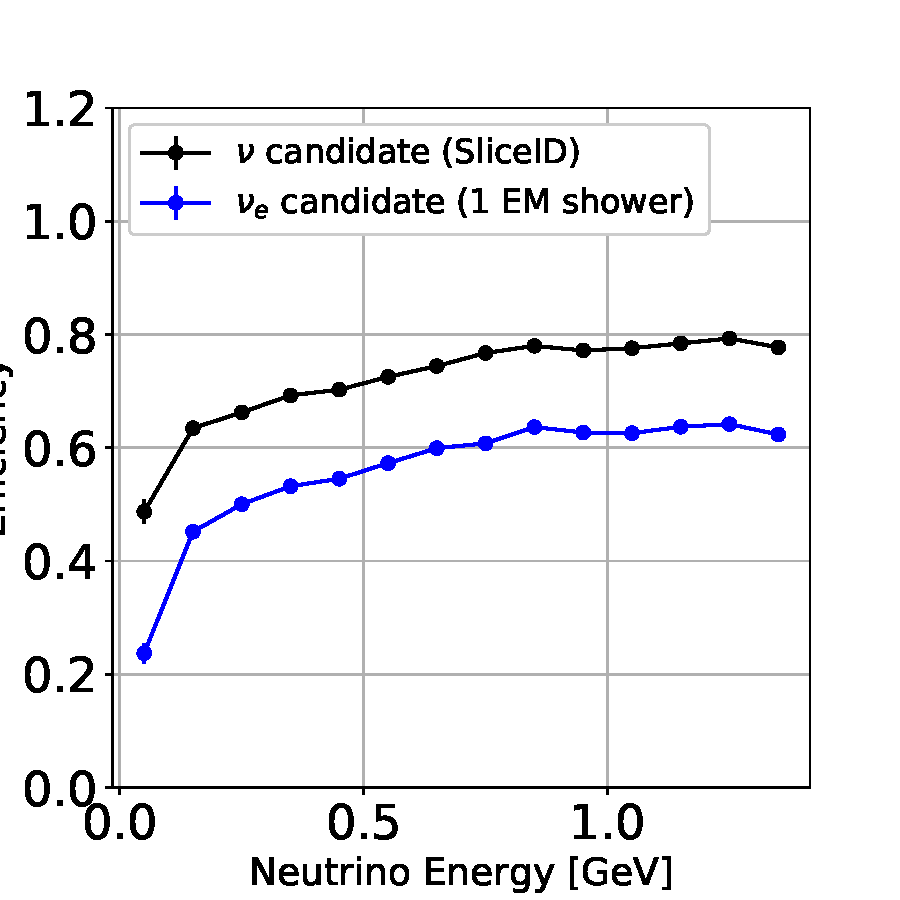
\includegraphics[width=1.00\textwidth]{nureco/nureco_RUN1.pdf}
    \caption{\label{fig:nuereco:eff} $\nu_e$ reco eff.}
    \end{subfigure}
    \begin{subfigure}[b]{0.31\textwidth}
    \centering
    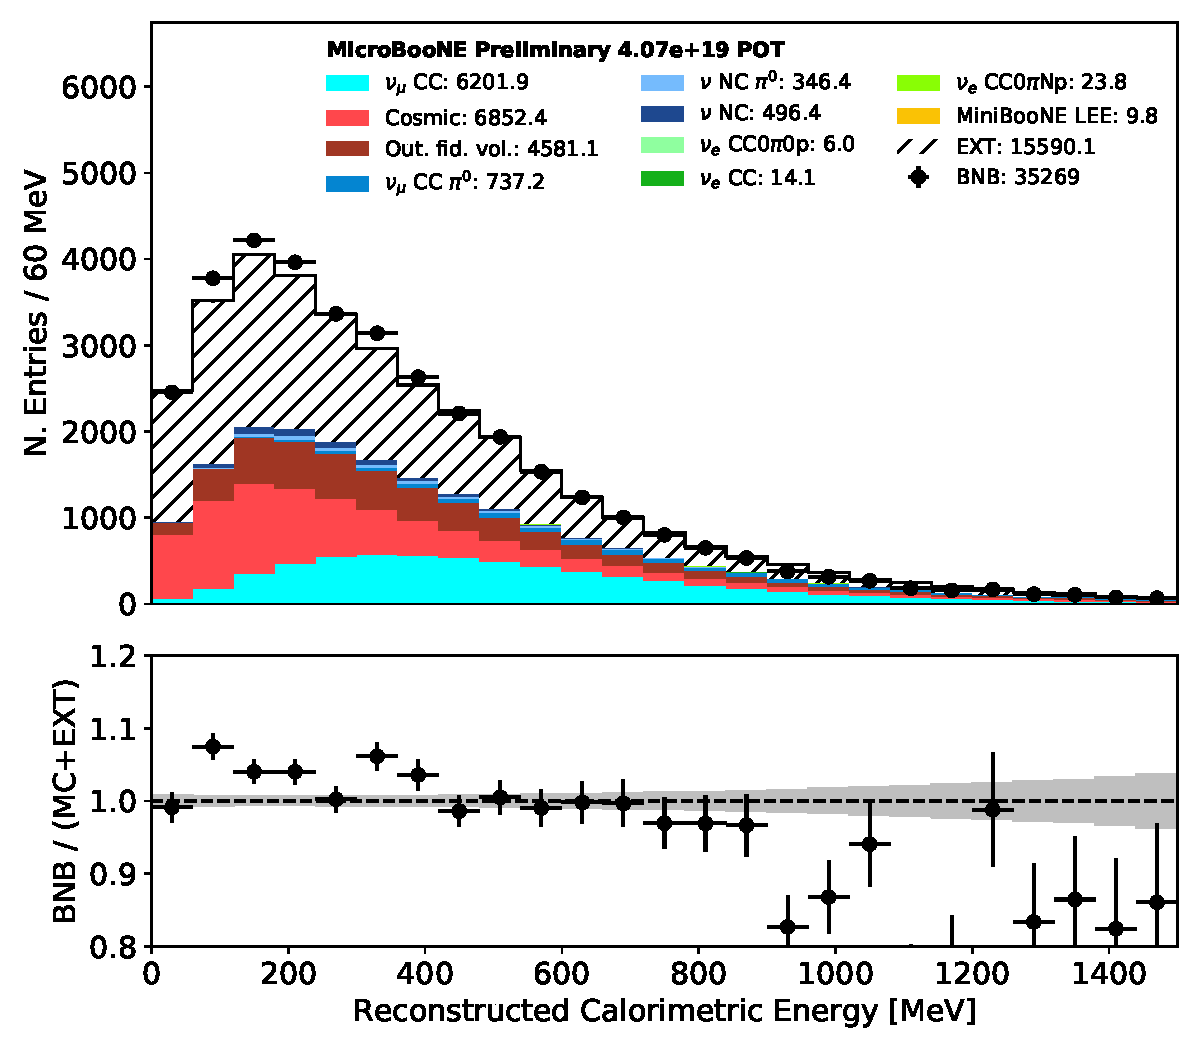
\includegraphics[width=1.00\textwidth]{nureco/NeutrinoEnergy2_01152020.pdf}
    \caption{\label{fig:nuereco:sliceid} after \texttt{SliceID}}
    \end{subfigure}
    \begin{subfigure}[b]{0.31\textwidth}
    \centering
    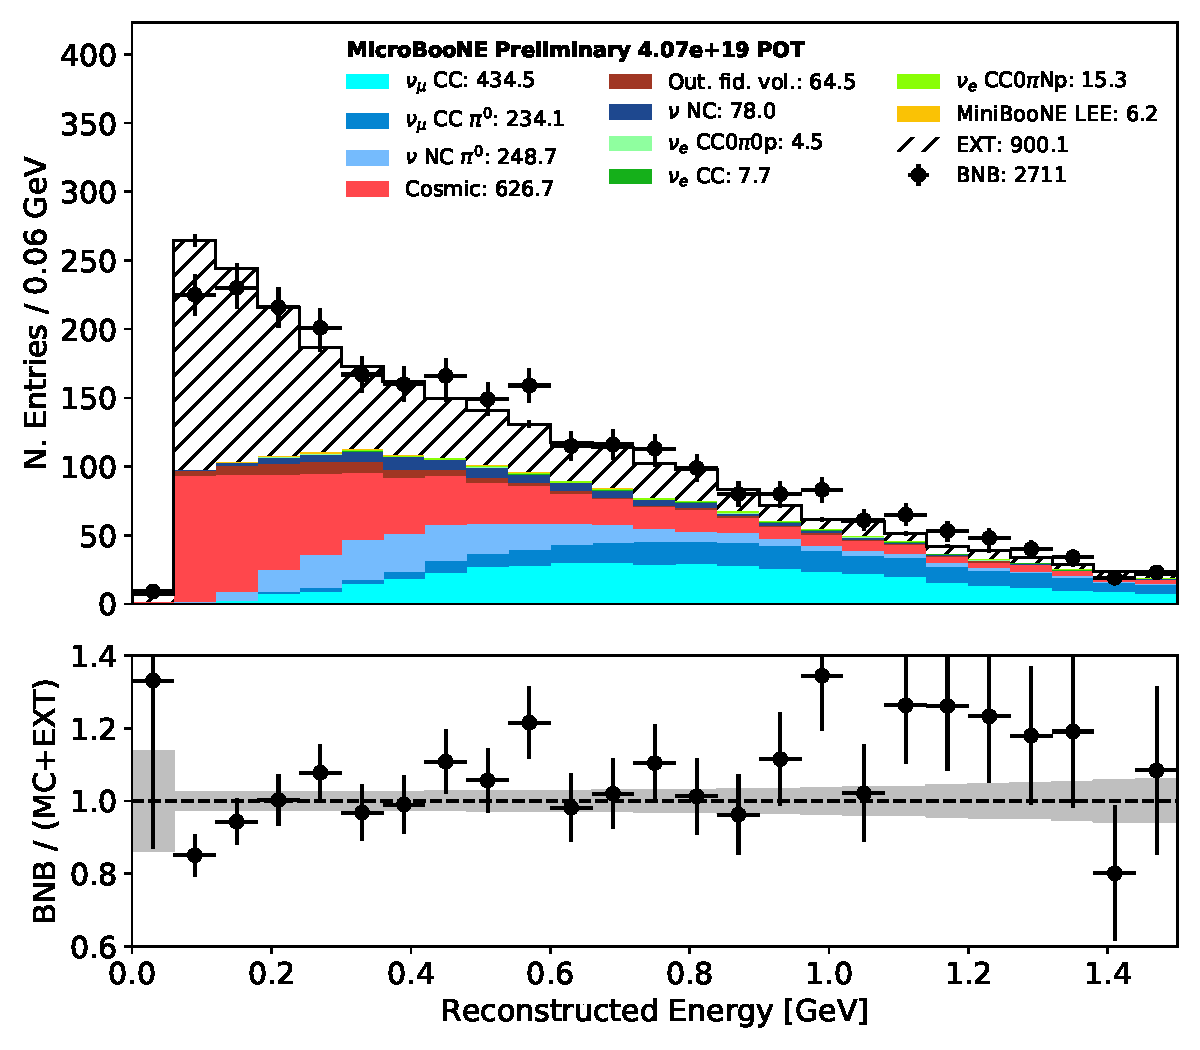
\includegraphics[width=1.00\textwidth]{nureco/reco_e_01152020.pdf}
    \caption{\label{fig:nuereco:shower} after shower requirement}
    \end{subfigure}
\caption{\label{fig:nuereco} \textcolor{blue}{ Y axis of figure a is cut off}}
\end{center}
\end{figure}

\par The next step in the analysis demands the development of a selection capable of isolating $\nu_e$ interactions rejecting the two order of magnitude larger background rates from $\nu_{\mu}$ neutrinos. This selection will make use of PID and topological information described in the next sections. The strong level of background rejection needed to isolate signal events will inevitably lead to a lower selection efficiency.

\subsection{Particle Identification \textcolor{green}{Nico, reviewed by David,Elena}}
% GC: this part is now in the previous subsection
%In the neutrino slice, every PFParticle is reconstructed in three different ways:
%\begin{itemize}
%    \item Track, using the standard Pandora Track reconstruction
%    \item Shower, using the standard Pandora Shower reconstruction (is there any modification on top of this?)
%    \item Track-fitted shower, using a dedicated track fitting tool which aims at identifying the main branch of %the shower and fit it as a track. As a result, all the tools developed for the track become available for the %tracks too. For example, for each track-fitted shower, a recob::track and a anab::calorimetry objects are available.
%\end{itemize}
Particle identification is performed with different tools depending \textcolor{blue}{on whether the particle is selected as a track- or shower-candidate \st{the type of candidate a given PFParticle has been selected as}.
If the PFParticle has been selected as a \st{muon or proton candidate, so as a} track-like object}, the identification is performed using the Calorimetry Likelihood tool, which results in the variable Log Likelihood Ratio PID (LLR), see section~\ref{subsec:loglikelihoodpid}.
If the PFParticle has been selected as an electron or photon candidate, the identification is performed using several variables described in \ref{subsec:egammaspearation}.
%It is noteworthy that this particle identification consists of one or multiple variables, available for the specific PFParticle, that may or may not depend on \textcolor{blue}{additional information from} the rest of the slice. 
%For example, the shower d$E$/d$x$ depends only on the PFParticle itself, whereas the track-shower separation relies also on additional objects identified in the slice.
Notably, additional information provided by the rest of the slice may be used for the particle identification 
depending on the specific PFParticle. For example, while the shower d$E$/d$x$ depends only on the PFParticle itself, the track-shower separation relies also on additional objects identified in the slice.

When choosing the cut values for PID variables, we account not only for the efficiency and mis-identification achievable to distinguish two kinds of particles (e.g. electrons from photons), but also for the mixture of backgrounds specific to the considered topology: e.g. \textcolor{blue}{add example}. 

%The value of the cuts applied on these variables depends not only on the general level of efficiency and mis-identification achievable to distinguish two kind of particles (electrons from photons, for example), but also on the mixture of backgrounds specific to selection the analyzer is performing.





\subsubsection{Log Likelihood Ratio  PID \textcolor{green}{Nico, P.R. David, Elena}}
\label{subsec:loglikelihoodpid}

For track-like particles, the particle identification is performed looking at the profile of the deposited charge per unit length (d$E$/d$x$). The scope of track PID is to identify the particle type which originated a given track object. In this analysis, we limit PID to a binary classification problem, i.e.  how to distinguish protons from muons. We disregard further classification because kaons are rarely produced in neutrino interactions at the energy of interest, whereas pions are very difficult to distinguish from muons using calorimetry information only.
Additional information, such as possible hadronic reinteractions or Michel electrons, can be powerful to perform particle identification but is not leveraged in this analysis.

The expected distribution of the $dE/dx$ is modeled for each particle type and for each plane, as a function of two variables: the residual range ($rr$), and the pitch as
\[ p(dE/dx | \text{type}, \text{plane}, \text{rr}, \text{pitch}). \]
The residual range is the distance of a given space point from the end of the track, measured along the track trajectory, while the pitch is the length over which the charge measured on a given wire has been deposited.
The expected distribution is modeled for each plane independently, and for the two kinds of particles under study, protons and muons.
Multiple effects enter in the model of this distribution.
The first effect is what we want to leverage:  the average d$E$/d$x$ at a given residual range depends on the particle's mass, as seen by integrating the Bethe-Bloch function for different masses.
Secondly, the fluctuations of the d$E$/d$x$ depend on the pitch. These fluctuations are intrinsically stochastic: the longer the length over which the charge is averaged, the smaller the fluctuations.
Furthermore, detector effects such as recombination, signal deconvolution, and hit reconstruction add a non-linear response and smearing; this response depends on both the true deposited charge and the pitch, and lacks an analytic model. For this reason, the expected distribution of $dE/dx$ is built starting from the simulation.
The performance of the particle identification improves as the model for the  $dE/dx$ distribution becomes more accurate.
The model for $dE/dx$ is built by considering well reconstructed tracks\footnote{ We define a ``well reconstructed track" a track whose completeness and purity are both above 90\%, where completeness measures how much of the true particle's  deposited charge is reconstructed in the track and purity measures how little spurious charge enters the track reconstruction. }, well contained within a fiducial volume, and backtracked to protons and muons.
The binning of the probability density function (pdf) is the following:
\begin{itemize}
    \item $dE/dx$: $[0, 0.5, 1, 1.5, 2, 2.5, 3, 3.5, 4, 4.5, 5, 5.5, 6, 6.5, 7, 7.5, 8, 9, 10, 12, 15, 20, 25, 30, 35, 40, 45, 50]$ MeV/cm
    \item residual range: $[0., 2, 4, 7, 10, 15, 20, 30, 50, 100, 300, 2000]$ cm
    \item pitch: $[0.3, 0.6, 1, 1.5, 3, 30]$ cm
\end{itemize}
A couple of examples of the pdf are provided in figure \ref{fig:llr_pid_pdf_example}, for two different bins in residual range and pitch.

\begin{figure}[ht] 
\begin{center}
    \begin{subfigure}[b]{0.48\textwidth}
    \centering
    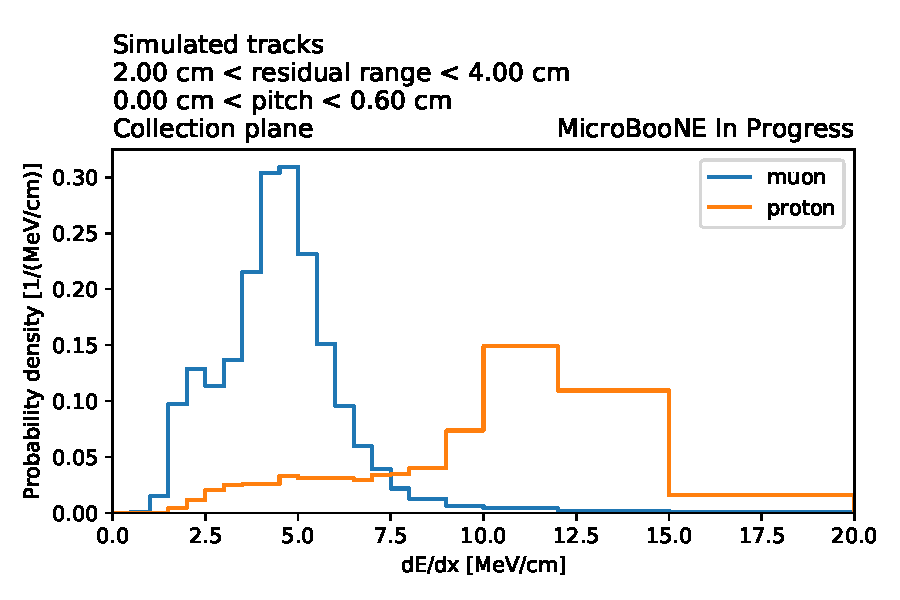
\includegraphics[width=1.00\textwidth]{llrpid/plane_2_rr_30_pitch_03.pdf}
    \end{subfigure}
    \begin{subfigure}[b]{0.48\textwidth}
    \centering
    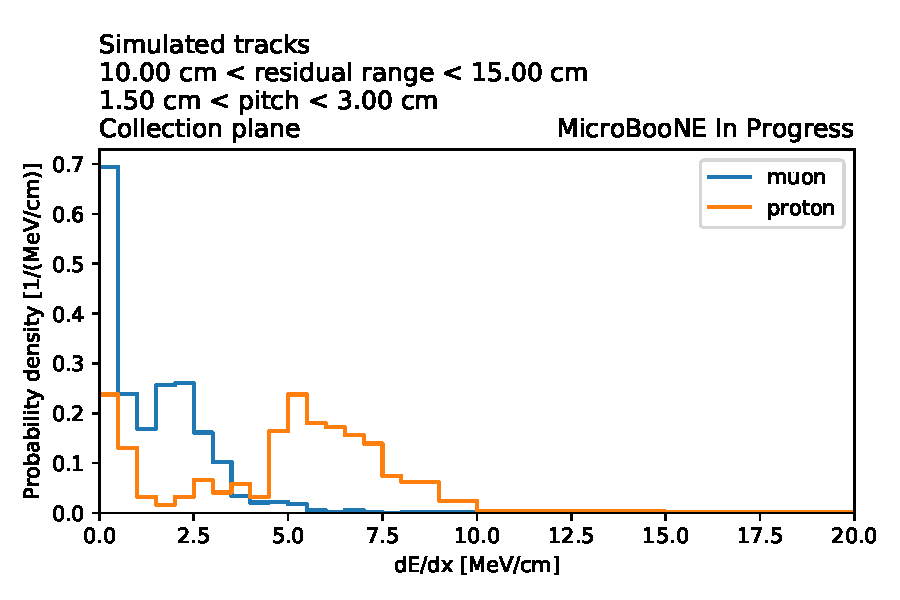
\includegraphics[width=1.00\textwidth]{llrpid/plane_2_rr_125_pitch_225.pdf}
    \end{subfigure}
\caption{Comparison of the expected distribution of $dE/dx$ for muons (blue) and protons (orange), for two different bins in residual range and pitch (left and right).}
\label{fig:llr_pid_pdf_example}
\end{center}
\end{figure}

For a given track, we consider the calorimetry objects on all three planes. For each plane, the $dE/dx$, residual range, and pitch vectors are used to compute the likelihood of each particle type,
\[ \mathcal{L}(\text{type} | \text{plane}, dE/dx_{i = 1, ..., N},   \text{rr}_{i = 1, ..., N}, \text{pitch}_{i = 1, ..., N}) = \prod_{i=1}^N p(dE/dx_i | \text{type}, \text{plane}, \text{rr}_i, \text{pitch}_i) \]
where the index $i=1, ..., N$ runs over each hit for the considered plane.
The combination of the three planes happens in a straightforward way, by taking the product of the three likelihoods, or summing up the log-likelihoods,
\[ p(dE/dx | \text{type}, \text{plane}, \text{rr}, \text{pitch}). \]
In order to perform the classification task, the likelihood ratio test statistic is chosen:
\[ T(dE/dx, \text{rr}, \text{pitch}) = \mathcal{L}(\text(muon)| dE/dx, \text{rr}, \text{pitch}) /  \mathcal{L}(\text(proton)| dE/dx, \text{rr}, \text{pitch}). \]
An example of the distribution of these variable, normalized between -1 and 1, is given in figure \ref{fig:llr_pid_uvy_example}, for tracks contained in a fiducial volume, and backtracked to muon, proton, or cosmic.

The likelihood ratio, as defined above can be proven to be the most powerful statistical test, i.e. the one with the smallest mis-identification rate for any given value of the efficiency.
Any mis-modeling in the simulation used to build the likelihood produces a loss of power, as the test would not be the most powerful one.
Systematic uncertainties arise from the fact that the measured distribution of $dE/dx$ in the data may differ from the simulation, or because the properties of the tracks we consider may not be properly simulated, such as angular or length distributions.
This behaviour is qualitatively present in all the PID methods.

In a MC sample of contained protons and muons used to test the performance, this PID variable is able to reach 94\% muon efficiency, with 10\% proton mis-ID rate.

\begin{figure}[ht] 
    \centering
    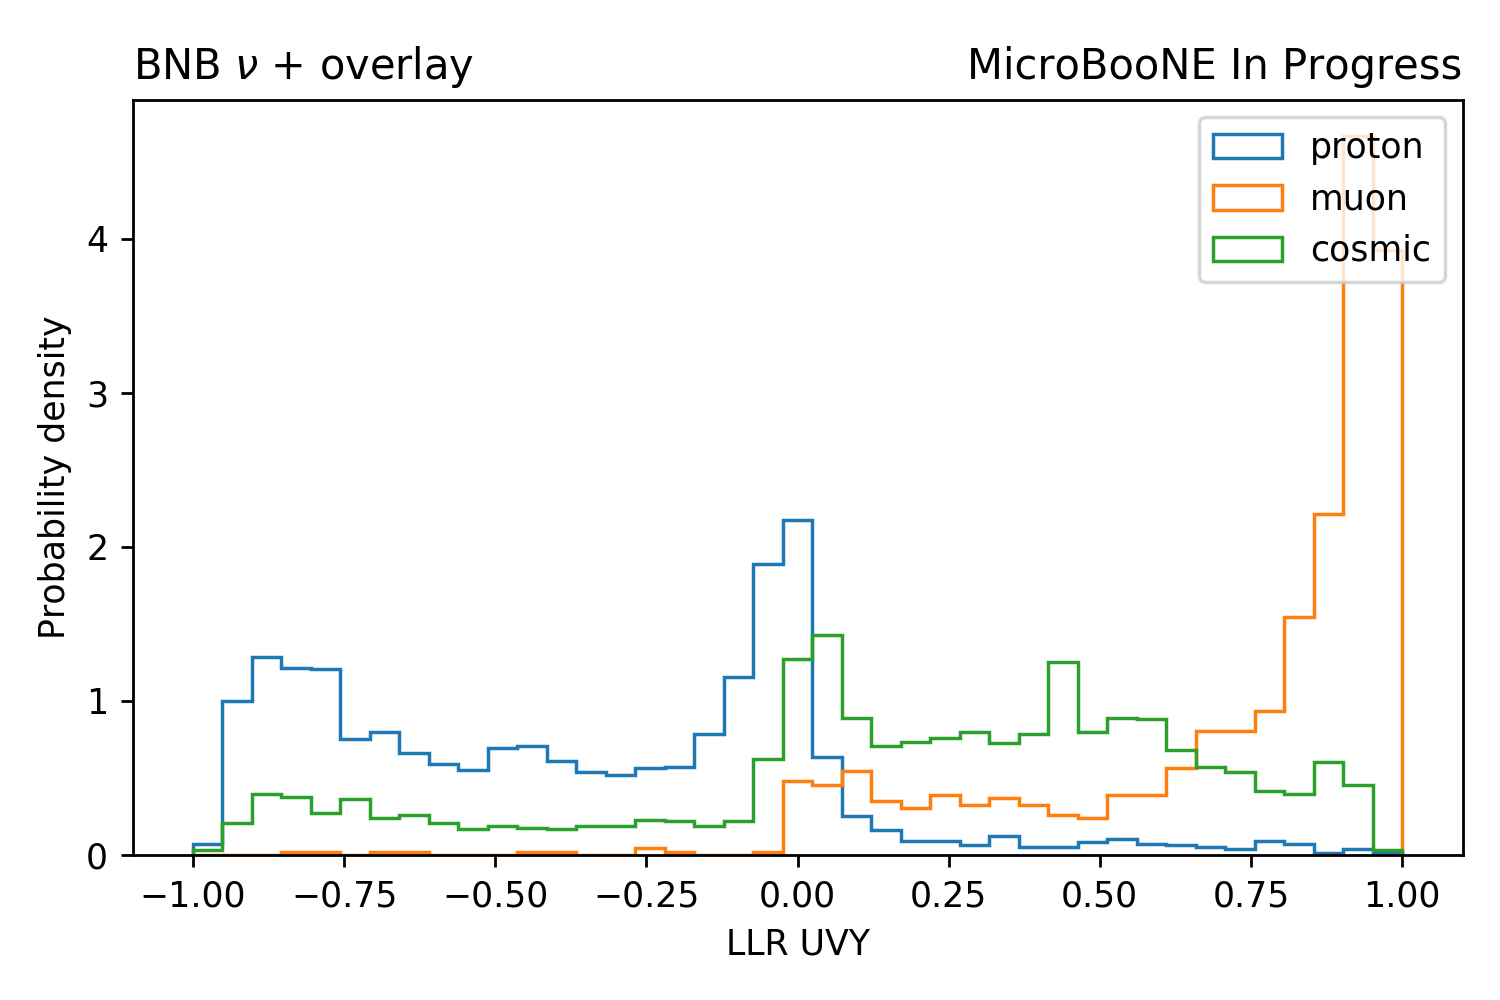
\includegraphics[width=0.7\textwidth]{llrpid/llr_012_n.png}
    \caption{Distribution of the log-likelihood-ratio PID variable for tracks well contained in a fiducial volume, and backtracked to muon (orange), proton (blue), or cosmic (green).}
    \label{fig:llr_pid_uvy_example}
\end{figure}




\subsubsection{$e$/$\gamma$ Separation \textcolor{green}{David, P.R Elena}}
\label{subsec:egammaspearation}
\par Distinguishing electron from photon EM-showers is one of the crucial steps required to perform a measurement of $\nu_e$ interactions in the BNB beam. Photon backgrounds to a $\nu_e$ measurement are largely caused by neutrino interactions with $\pi^0 \rightarrow \gamma\gamma$ in the final state; this topology dominates the $\nu_e$ event rate by approximately an order of magnitude. Three key features distinguish events with $\pi^0$ induced photon showers from $\nu_e$ interactions: (a) the presence of two final state EM showers. (b) the non-zero conversion distance separating the neutrino interaction vertex from the shower start point, and (c) the calorimetric separation via $dE$/$dx$ due to the overlapping ionization segment of $e^+$/$e^-$ pair-conversions through which most $\gamma$ showers manifest themselves. Figure~\ref{fig:egammasep} shows how, at reconstruction level, each of these features can aid in $e$/$\gamma$ separation. This section describes how each of the items above is utilized in the analysis on a technical level, what performance is obtained, and what challenges (both physics- and reconstruction-driven) are encountered when leveraging these variables.

\begin{figure}[ht] 
\begin{center}
    \begin{subfigure}[b]{0.31\textwidth}
    \centering
    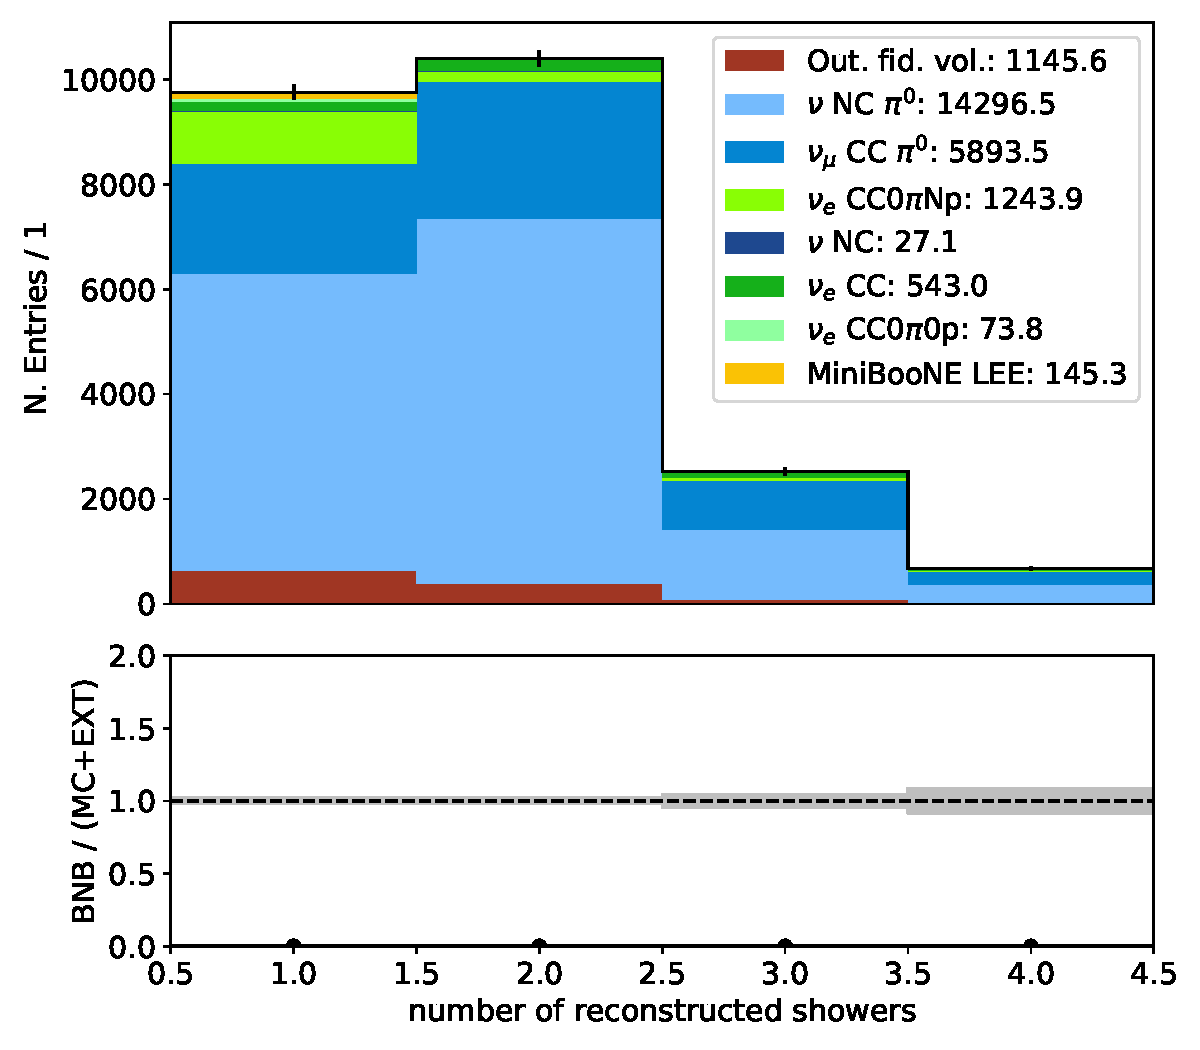
\includegraphics[width=1.00\textwidth]{egamma/n_showers_contained_01022020.pdf}
    \caption{number of reconstructed showers}
    \end{subfigure}
    \begin{subfigure}[b]{0.31\textwidth}
    \centering
    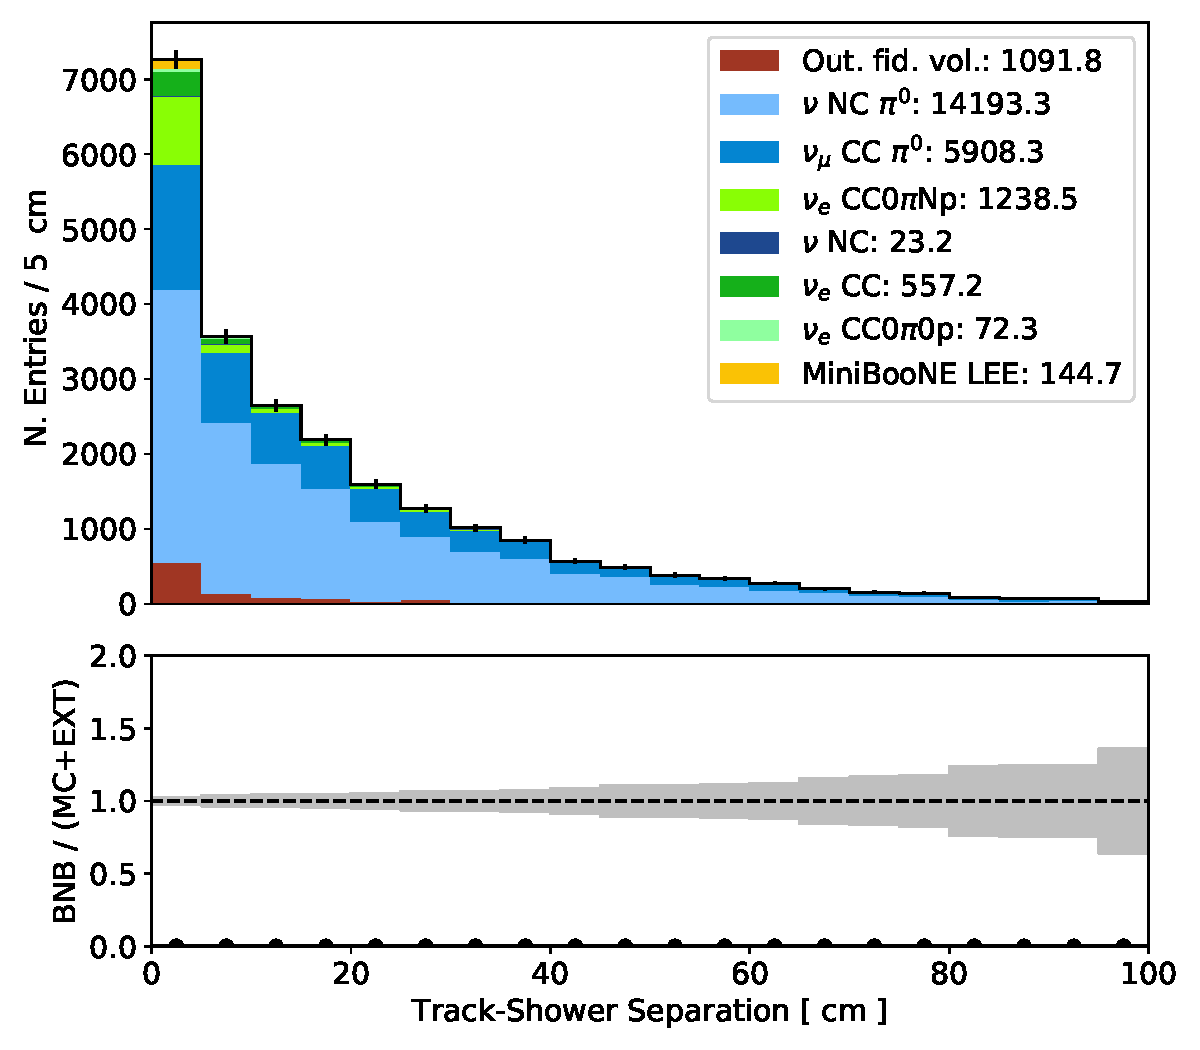
\includegraphics[width=1.00\textwidth]{egamma/tksh_distance_01022020.pdf}
    \caption{track-shower separation}
    \end{subfigure}
    \begin{subfigure}[b]{0.31\textwidth}
    \centering
    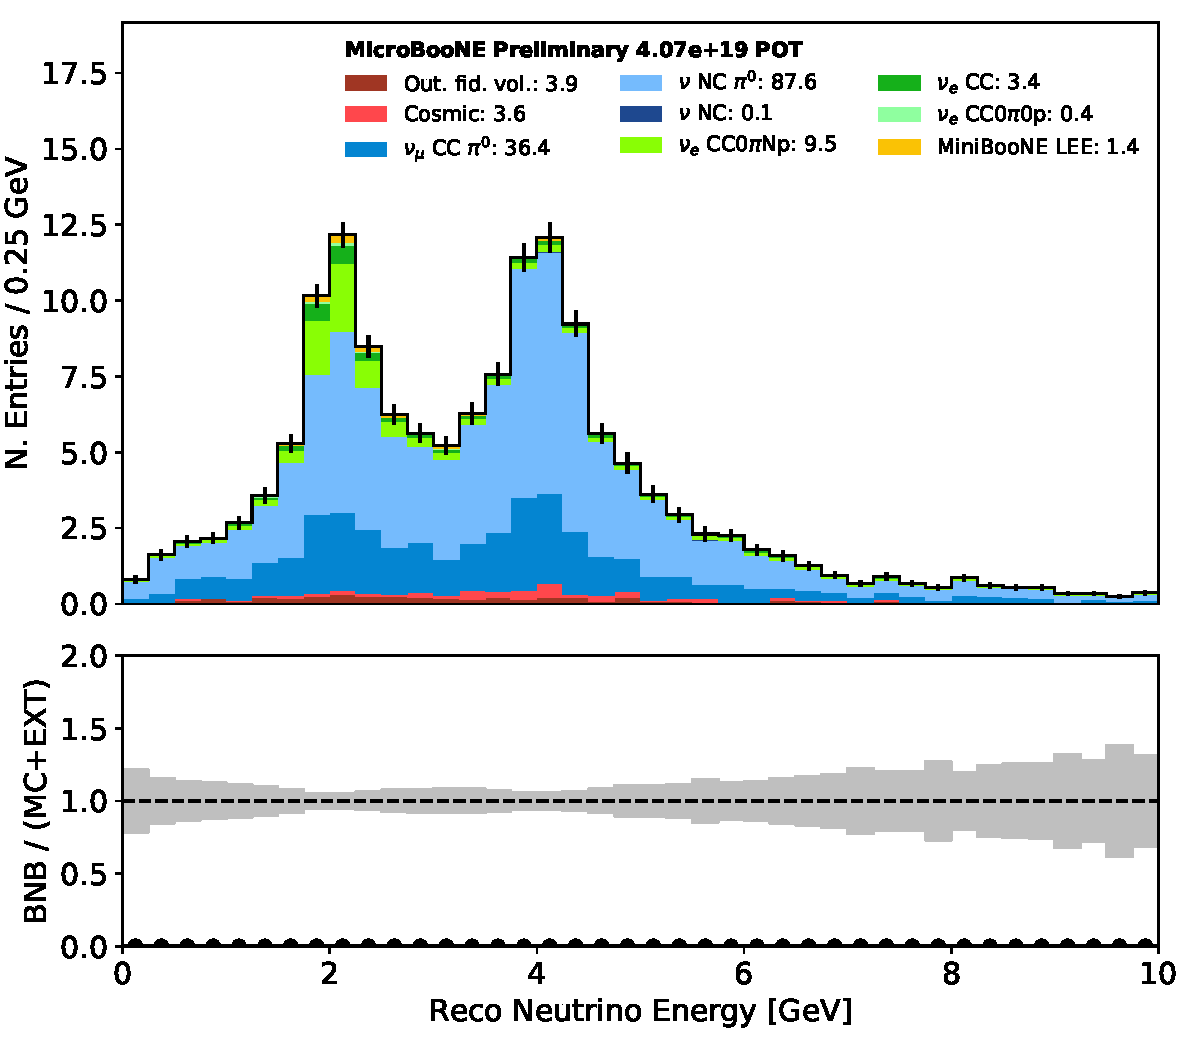
\includegraphics[width=1.00\textwidth]{egamma/shr_tkfit_dedx_Y_01192020.pdf}
    \caption{\label{fig:egammasep:dedx} reconstructed shower $dE$/$dx$}
    \end{subfigure}
\caption{\label{fig:egammasep}Comparison of simulated $\nu_e$ (green) vs. $\nu_{\mu} \rightarrow \pi^0 + X$ (blue) for the three discriminating variables of (a) number of showers, (b) vertex distance, and (c) $dE$/$dx$. Distributions are POT-normalized but contain only $\nu_e$ or $\pi^0$ events (no on/off-beam data distributions).}
\end{center}
\end{figure}

\par \textbf{two-shower requirement} Requiring a single reconstructed shower retains 68\% of $\nu_e$ interactions (with no $\pi^0$ in the final state) while removing 61\% of $\nu_{\mu}$ events with at least one $\pi^0$ in the final state. The fraction of selected $\nu_e$s grows to 79\% when looking below 800 MeV of true energy (the focus of this analysis). Rejection of $\nu_e$s is largely due to events where the electron shower is reconstructed as two separate EM showers, often closely aligned in 3D. Events with final state $\pi^0$s are reconstructed with a single EM shower in the final state because either the second photon escapes the TPC active volume completely (irreducible) or because the second shower is not reconstructed. The dominant causes of this second case are (1) highly-boosted $\pi^0$ decays, in which two aligned photons are merged into one shower and (2) photons which go undetected, often low in energy (below 100 MeV). Additional discriminating variables which aim to recover the reconstruction-related mis-ID of (1) and (2) are utilized in the analysis and presented in Sec.~\ref{sec:nueselection:inputs}.
\par \textbf{track-shower separation} For events where hadronic activity at the neutrino interaction vertex (i.e. final-state protons) is visible, a clear gap between the vertex and the shower start-point can be used to reject $\gamma$ backgrounds. This is a powerful background mitigation tool in the 1$e$N$p$ $\nu_e$ selection. Two factors determine the performance of such a tool: the ability to detect protons and other hadronic activity at the vertex and the accuracy with which the shower start-point is reconstructed. The shower start-point reconstruction accuracy determines the level of background rejection obtainable, as $\gamma$ showers lead to an exponential conversion-distance distribution. \textcolor{blue}{A 1 cm vs. 5 cm track-shower separation cut leads to 95\% vs 74\% mis-ID respectively, but causes a drop in selection efficiency for 1$e$N$p$ events from 72\% to 28\%. I don't think I understand these numbers... because what  I'm understanding is not logical: if I reject events with a 1 cm or more gap, I keep 72\% of nues and 95\% of photons. If I reject events with a 5 cm or more gap, I keep only 28\% nue and 75\% photons. This is completely counter intuitive, what am I getting wrong?  } This is a consequence of the sub-optimal vertex reconstruction accuracy for low-energy $\nu_e$ interactions. In order to enhance the ability to isolate $\nu_e$ events in the 1$e$N$p$ selection through vertex-displacement, different metrics are used to measure the presence of a gap between an electron and proton candidate. These will be described in section~\ref{sec:nueselection:inputs}. It is important to note that this background mitigation strategy is not applicable to single-electron searches, which are an important contribution to $\nu_e$ interactions, especially in the low-energy regime.
\par \textbf{shower d$E$/d$x$} The majority of photons manifest themselves in the TPC through the ionization released by the $e^+$/$e^-$ pair produced via pair-conversion. The electron-positron pair is highly aligned and overlaps on the mm-scale, leading to a doubly-ionizing charge-segment compared to electron showers. To measure this, we use the track fit of the main shower trunk and the calorimetric tools as described in Sec.~\ref{sec:tkshreco}. 
%with a modified version of the MicroBooNE track-fitter~\cite{bib:shrtrackfitter} and for each point along a track the d$Q$/d$x$  and distance from the shower-start are recorded using MicroBooNE's Calorimetry module. This procedure allows to accurately measure d$x$, including small deflections due to the electron's trajectory and SCE offsets, and d$Q$, by incorporating MicroBooNE's full position- and field-dependent relative and absolute charge calibration. From d$Q$/d$x$, d$E$/d$x$ is calculated assuming a fixed recombination correction assuming 2.1 MeV/cm energy loss, but accounting for local variations in the electric field. 
The distinctive 4 MeV/cm population expected for $\gamma$ showers is visible in figure~\ref{fig:egammasep:dedx}. The main limitation to $e$/$\gamma$ separation via d$E$/d$x$ is the large fraction of photons reconstructed with a d$E$/d$x$ of less then 3 MeV/cm (23\% of $\pi^0$ events fall in the 1-3 MeV range). This is due both to mis-reconstructed events, for which the start-point is incorrectly reconstructed by more than one or two cm, and to events where the photon shower's energy loss-profile is not as clearly distinguishable from that of a single electron. While the relative contribution of these two sources is still under determination, the second causes a significant mis-ID rate, and is largely associated to lower-energy $\gamma$ showers for which the production of a highly asymmetric electron-positron pair where one of the electrons is barely visible is more frequent. The impact of shower energy on the measured d$E$/d$x$ for a $\gamma$ shower is shown in figure~\ref{fig:dedxgammas:energy}. Below 100 MeV, where most $\gamma$ showers in the BNB are produced, the reconstructed d$E$/d$x$ is electron-like. The impact of distance from the shower start-point on whether d$E$/d$x$ is reconstructed to be 2 or 4 MeV/cm is also important, as can be seen in figure~\ref{fig:dedxgammas:dist}. This is particularly true for low-energy asymmetric pair-production events, and motivates utilizing 
d$E$/d$x$ information at different distances from the shower start-point for $e$/$\gamma$ separation.
\begin{figure}[H] 
\begin{center}
    \begin{subfigure}[b]{0.45\textwidth}
    \centering
    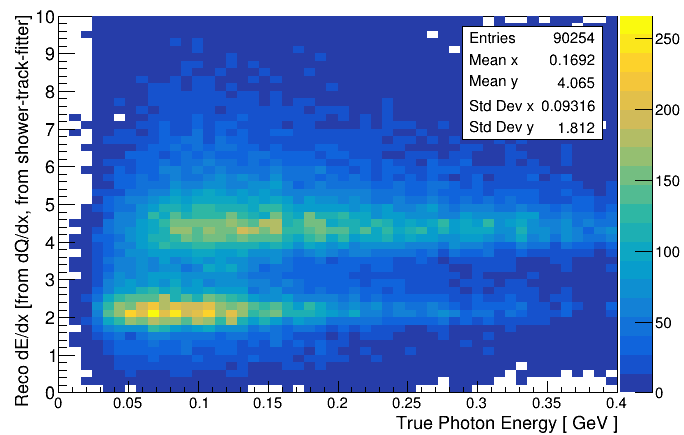
\includegraphics[width=1.00\textwidth]{egamma/dedx_vs_energy_gamma.png}
    \caption{\label{fig:dedxgammas:energy} d$E$/d$x$ vs. distance from shower start-point for $\gamma$ showers \textcolor{blue}{wrong caption}}
    \end{subfigure}
    \begin{subfigure}[b]{0.45\textwidth}
    \centering
    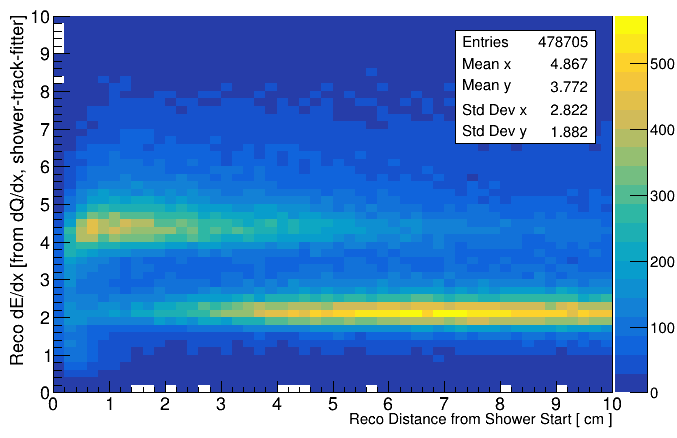
\includegraphics[width=1.00\textwidth]{egamma/dedx_vs_dist_gamma.png}
    \caption{\label{fig:dedxgammas:dist} d$E$/d$x$ vs. distance from shower start-point for $\gamma$ showers}
    \end{subfigure}
\caption{\label{fig:dedxgammas}}
\end{center}
\end{figure}



%\newpage

\subsection{Energy Reconstruction \textcolor{green}{Giuseppe + David... (PR Elena)}}
\label{sec:ereco}
\par Energy reconstruction is performed thought calorimetry for EM showers and through a measurement of a track's range for contained muons and protons. For \textcolor{blue}{should we add "uncontained"} muons, multiple Coulomb scattering (MCS) is also used to estimate the muon energy. The energy resolution obtained for different particles is reported in table~\ref{tab:eres}. More information on each particle's energy resolution is reported in figure~\ref{fig:eres:particle} where the 2D reconstructed vs. true energy distribution (in log-scale) is shown on the left, next to a plot of energy resolution vs. true energy on the right. The energy resolution reported here is obtained from a Gaussian plus one-sided exponential fit to the distribution $[E_{\rm reco}-E_{\rm true}] / E_{\rm true}$, see figures \ref{fig:eres:elec:binned}. The resolution reported refers only to the Gaussian width $\sigma$ extracted in the fit, and therefore does not account for negative tails, which are significant in the case of EM shower energy reconstruction, and described below.


\begin{table}[H]
\centering
  \begin{tabular}{ | c | c |  }
    \hline
    particle & kinetic energy resolution  \\ \hline
    proton & 4\% at 100 MeV 1\% at 200 MeV \\ \hline
    muon (range) & 3\%  \\ \hline
    muon (MCS) & $\frac{4.7\%}{\sqrt{E/{\rm GeV}}} \otimes \frac{2.8\%}{E/{\rm GeV}} \otimes 0.0\% \text{\textcolor{blue}{this is fairly confusing, especially the 0.0\%, can we add a reference, or an explaination?}}$  \\ \hline
    electron & 15\%  \\
    \hline
    
  \end{tabular}
  \caption{\label{tab:eres} Energy resolution for different particle species.}
 \end{table}
 
 \par For EM showers, the calorimetric energy reconstruction response has a significant non-Gaussian component, as well as a large bias. Both effects are attributable to reconstruction effects associated with under-clustering of charge. The energy bias is found to be 20\% and approximately flat in energy, and motivates a definition of a corrected shower energy, defined as $E_{\rm corrected} = E_{\rm calorimetry} / 0.8$. The non-Gaussian response for EM energy reconstruction can be modeled through a Gaussian plus one-sided exponential distribution. Figure~\ref{fig:eres:elec:binned} shows in different bins of true energy the fractional energy response and a fit to a Gaussian plus one-sided exponential function. The residual energy bias, after the 20\% correction applied, is of order $3-8$\%. 
 
 \begin{figure}[ht]
\begin{center}
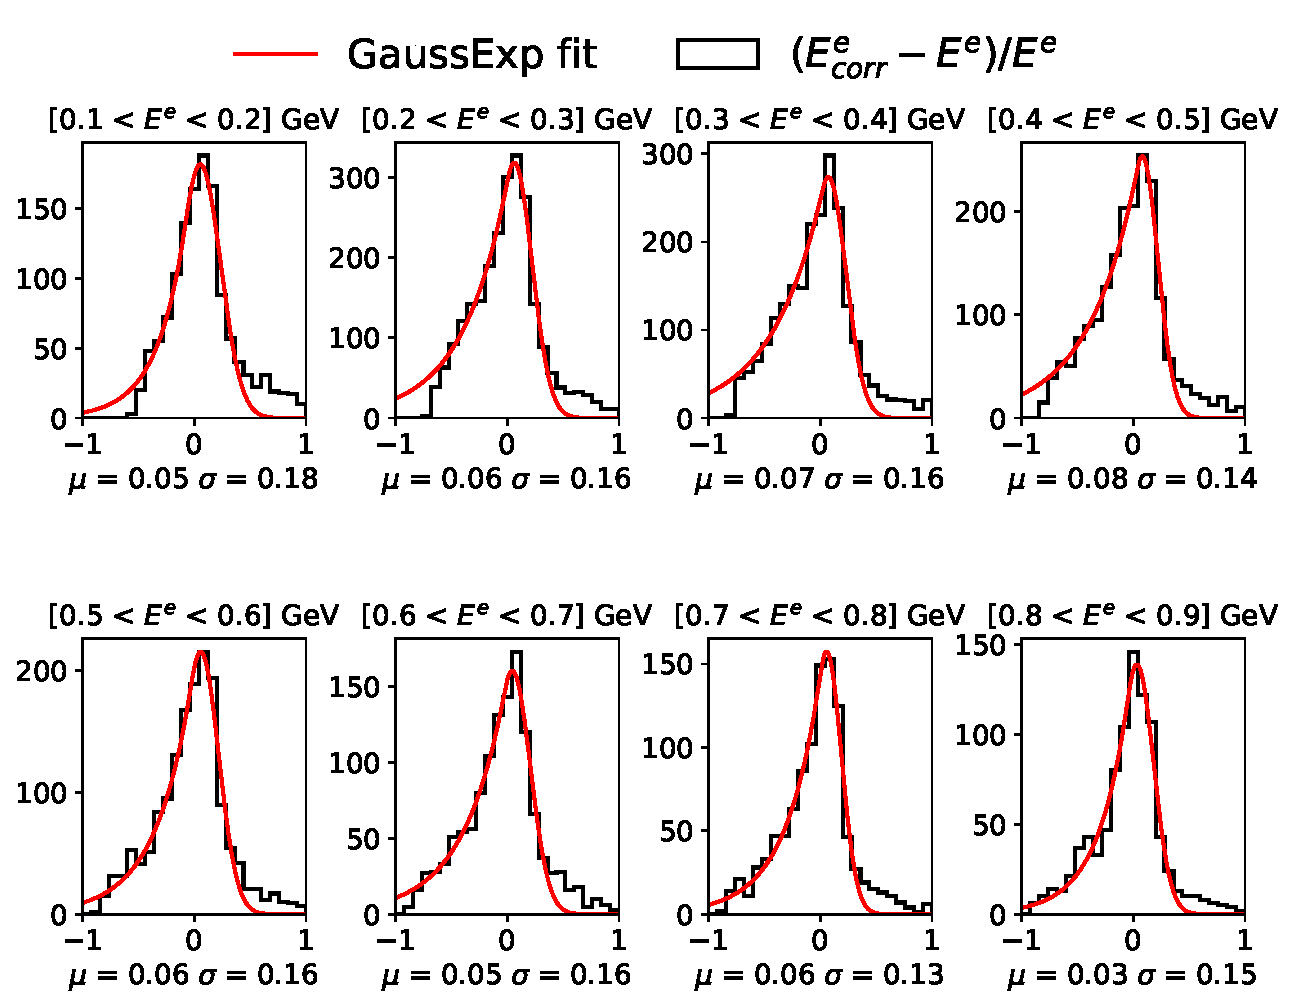
\includegraphics[width=0.75\textwidth]{ereco/elec_eres_binned.pdf}
\caption{\label{fig:eres:elec:binned}Energy resolution for electron showers.}
\end{center}
\end{figure}
 
\newpage

\begin{figure}[H] 
\begin{center}
    \begin{subfigure}[b]{0.4\textwidth}
    \centering
    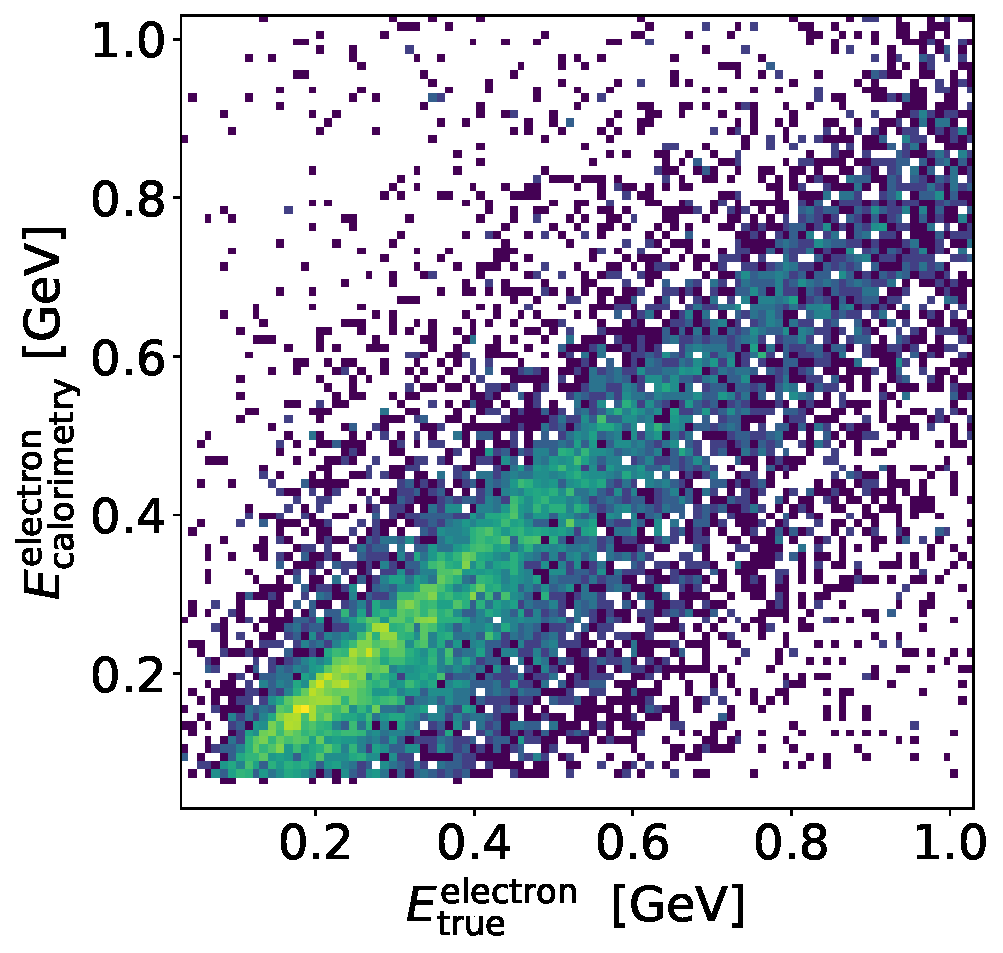
\includegraphics[width=1.00\textwidth]{ereco/electron_eres2D.pdf}
    %\caption{\label{fig:eres:elec:2d} }
    \end{subfigure}
    \begin{subfigure}[b]{0.38\textwidth}
    \centering
    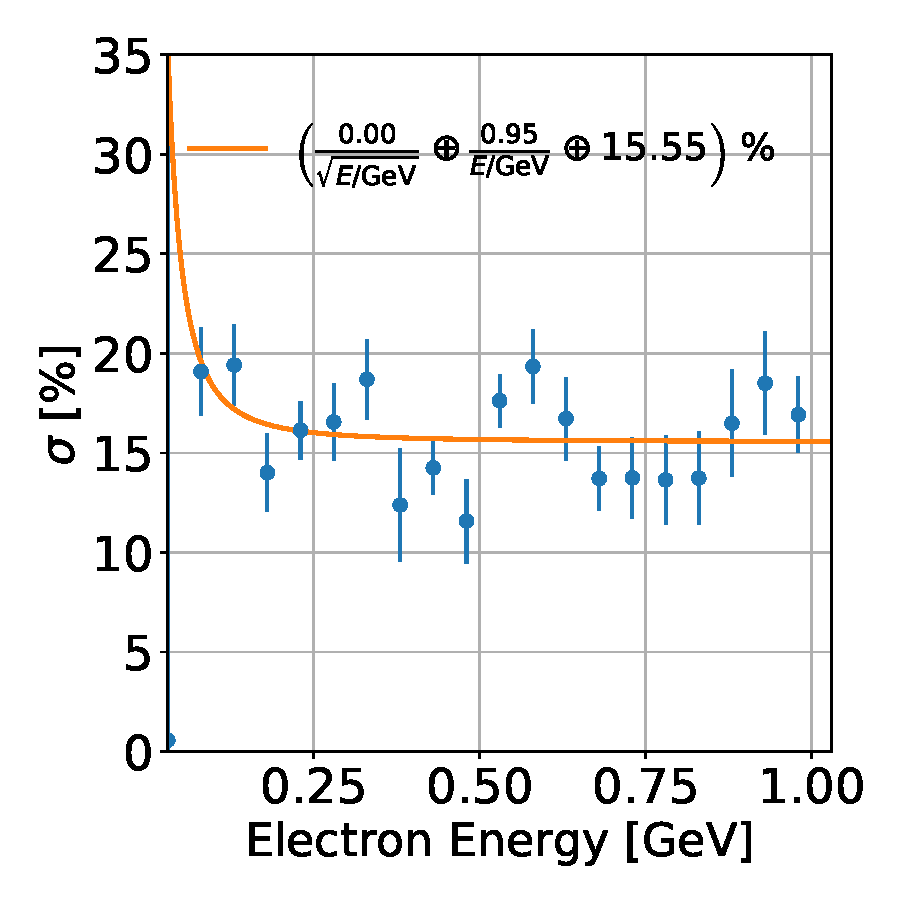
\includegraphics[width=1.00\textwidth]{ereco/elec_eres_vs_true.pdf}
    %\caption{\label{fig:eres:elec:vstrue} }
    \end{subfigure}
    \begin{subfigure}[b]{0.4\textwidth}
    \centering
    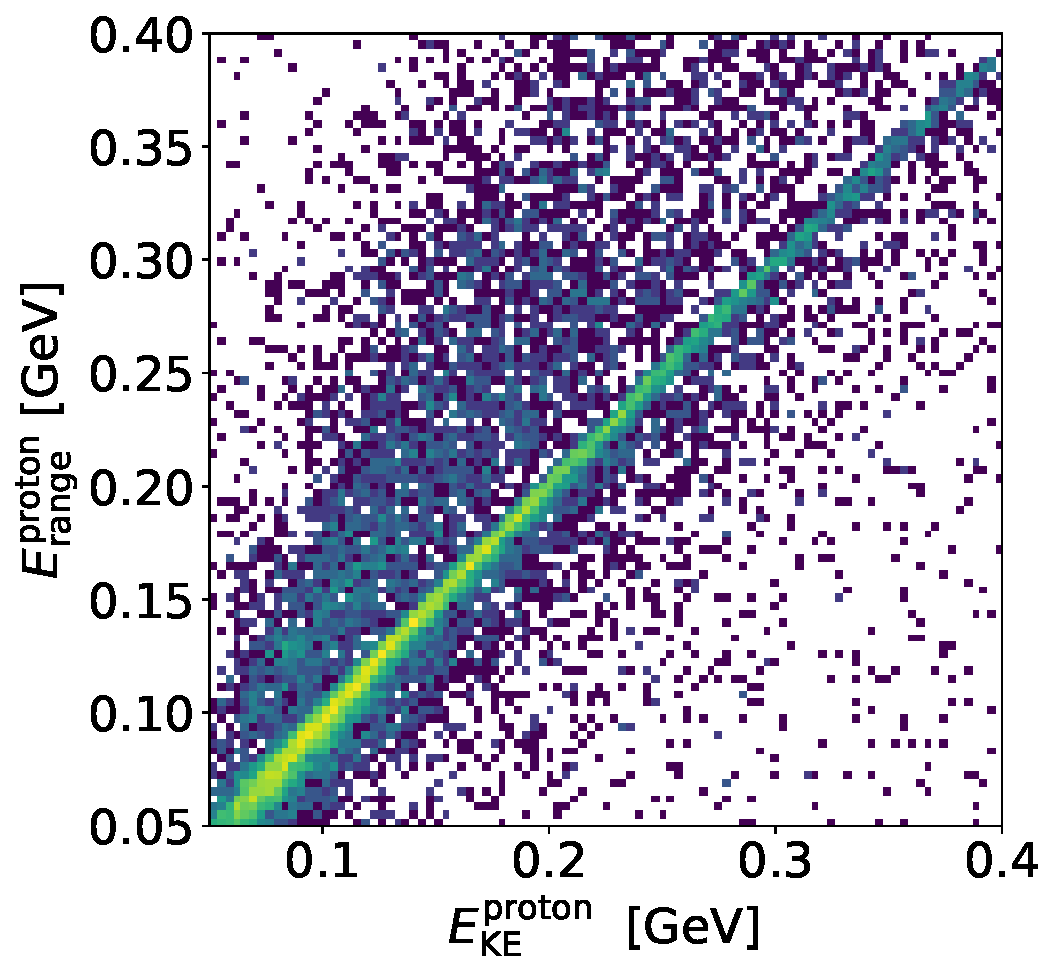
\includegraphics[width=1.00\textwidth]{ereco/proton_eres2D.pdf}
    %\caption{\label{fig:eres:proton:2d} }
    \end{subfigure}
    \begin{subfigure}[b]{0.38\textwidth}
    \centering
    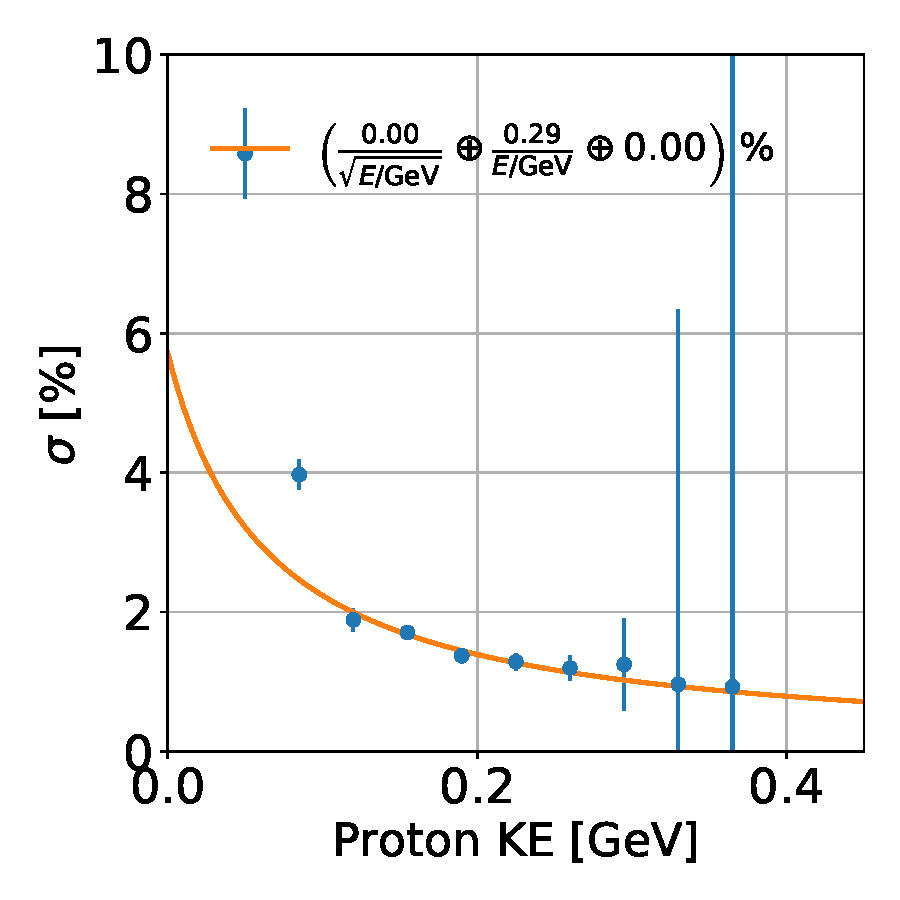
\includegraphics[width=1.00\textwidth]{ereco/proton_eres_vs_true.pdf}
    %\caption{\label{fig:eres:proton:vstrue} }
    \end{subfigure}
    \begin{subfigure}[b]{0.4\textwidth}
    \centering
    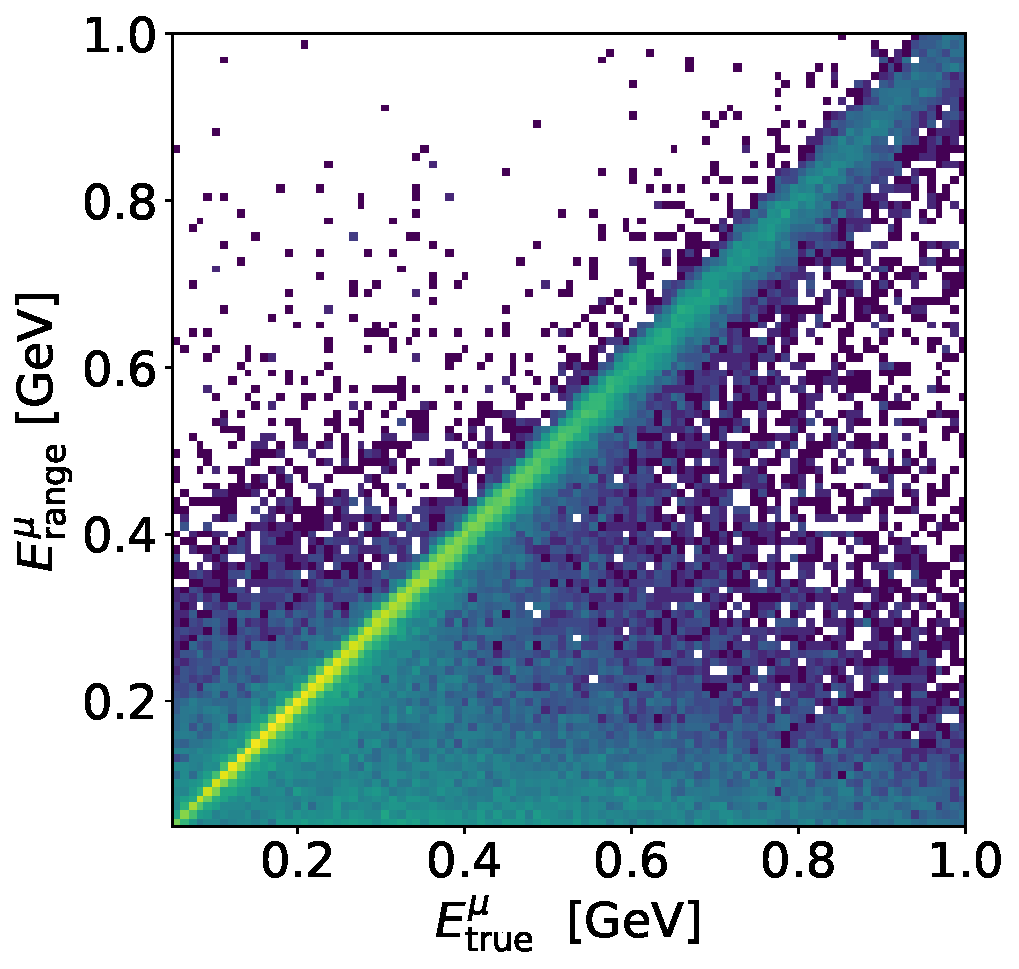
\includegraphics[width=1.00\textwidth]{ereco/muon_range_eres2D.pdf}
    %\caption{\label{fig:eres:muon:2d} }
    \end{subfigure}
    \begin{subfigure}[b]{0.38\textwidth}
    \centering
    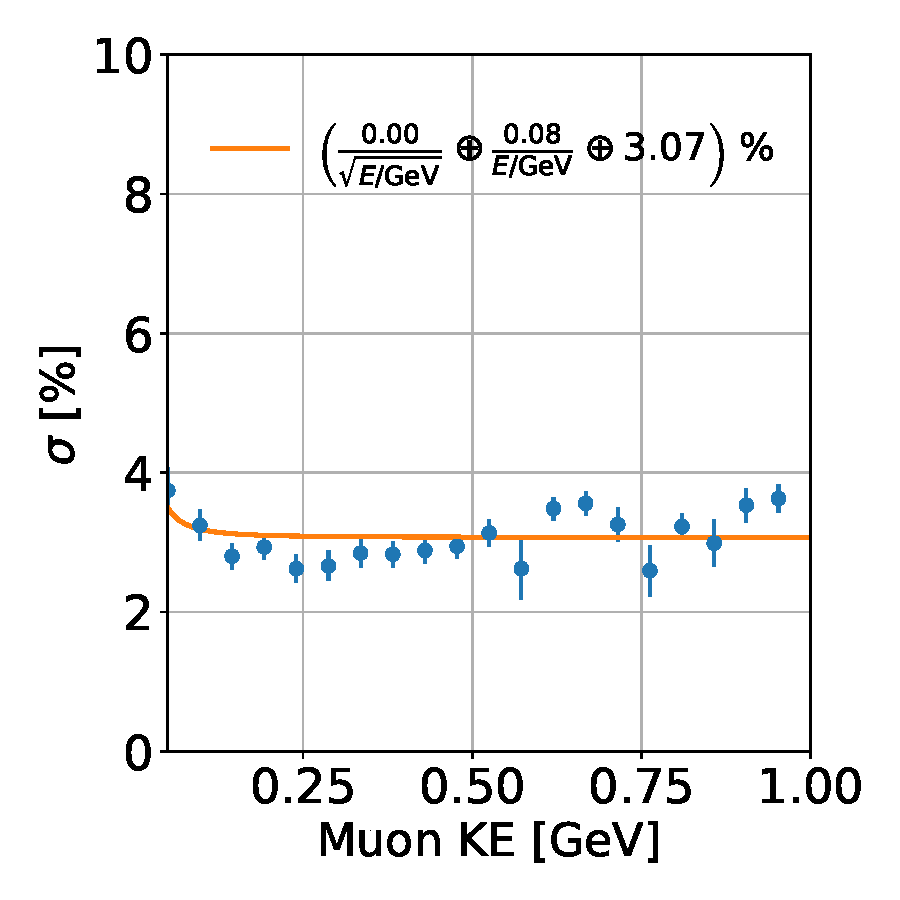
\includegraphics[width=1.00\textwidth]{ereco/muon_range_eres_vs_true.pdf}
    %\caption{\label{fig:eres:muon:vstrue} }
    \end{subfigure}
\caption{\label{fig:eres:particle}Energy resolution for electrons (top), protons (center) and muons (bottom). Left: reconstructed vs. true energy resolution (log-scale). Right: energy resolution from Gaussian fit to $[E_{\rm reco}-E_{\rm true}] / E_{\rm true}$.}
\end{center}
\end{figure}

\subsubsection{Neutrino Energy Reconstruction \textcolor{green}{Giuseppe + David, P.R. Elena}}

\par In this analysis, the energy reconstruction for neutrino interactions is performed through a sum of the visible energy of the various reconstructed final-state particles in the interaction. For $\nu_e$ events, the reconstructed energy is defined as:
\begin{equation}
    E_{\rm reco}^{\nu_e} = E_{\rm corrected}^{\rm electron} + \sum_{\rm tracks} E_{\rm range}^{\rm proton}.
\end{equation}{}
\textcolor{blue}{is this true also for nue inclusive?}.
For contained $\nu_{\mu}$ interactions, the reconstructed energy is defined as:

\begin{equation}
    E_{\rm reco}^{\nu_{\mu}} = E_{\rm range}^{\rm muon} + \sum_{\rm protons} E_{\rm range}^{\rm proton} + 0.105 \; GeV
\end{equation}{}

Figure~\ref{fig:eres:neutrino} shows the comparison between reconstructed energy and truth visible energy, which is defined as the sum of the lepton energy, pion energy (if present), and proton energy (for all protons above 40 MeV of KE). This comparison shows very accurate energy reconstruction for $\nu_{\mu}$ events \textcolor{blue}{uhm.... this is true up to a point: there's a tail for high numu visible and log numu range: does this come from events w/ non-contained muons?}. For $\nu_e$ interactions, with smearing dominated by the worse energy resolution of electron showers \textcolor{blue}{This sentence misses a verb}.

\begin{figure}[H] 
\begin{center}
    \begin{subfigure}[b]{0.4\textwidth}
    \centering
    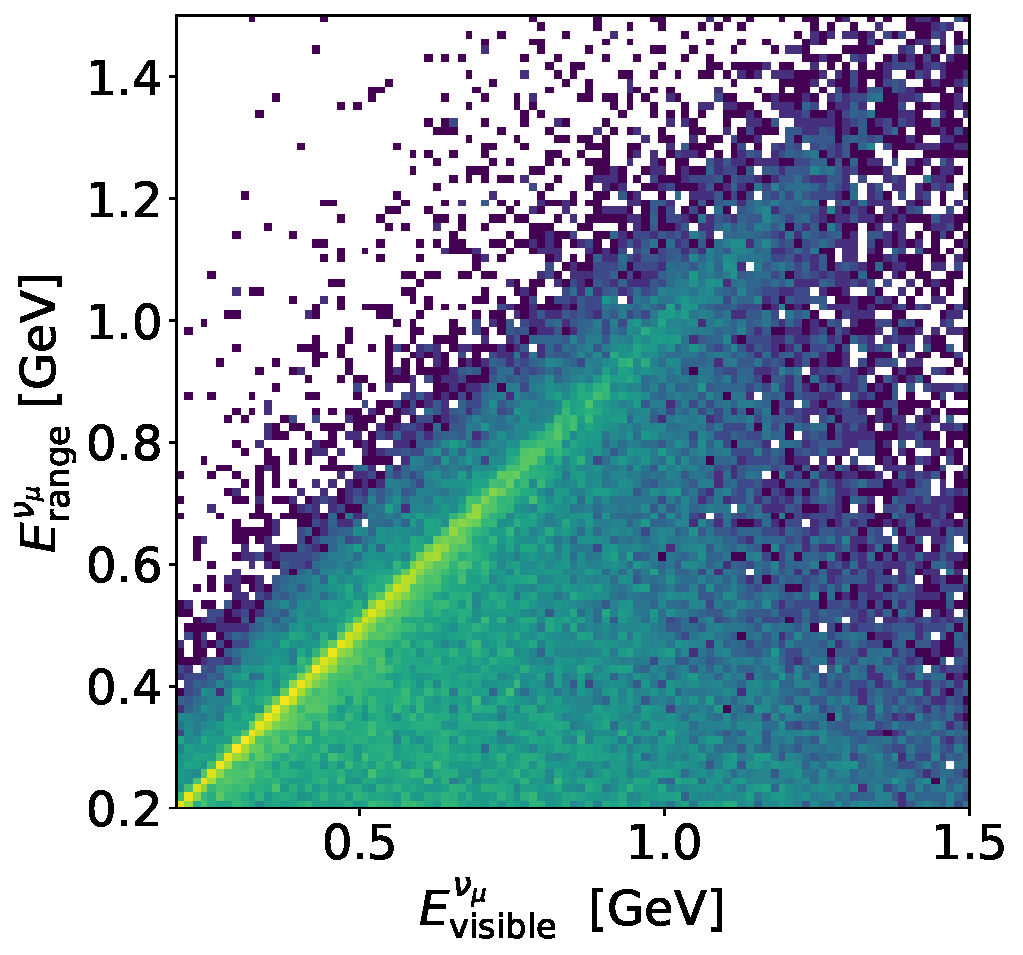
\includegraphics[width=1.00\textwidth]{ereco/numu_energy_visible_eres2D.pdf}
    \caption{\label{fig:eres:numu:2d} }
    \end{subfigure}
    \begin{subfigure}[b]{0.4\textwidth}
    \centering
    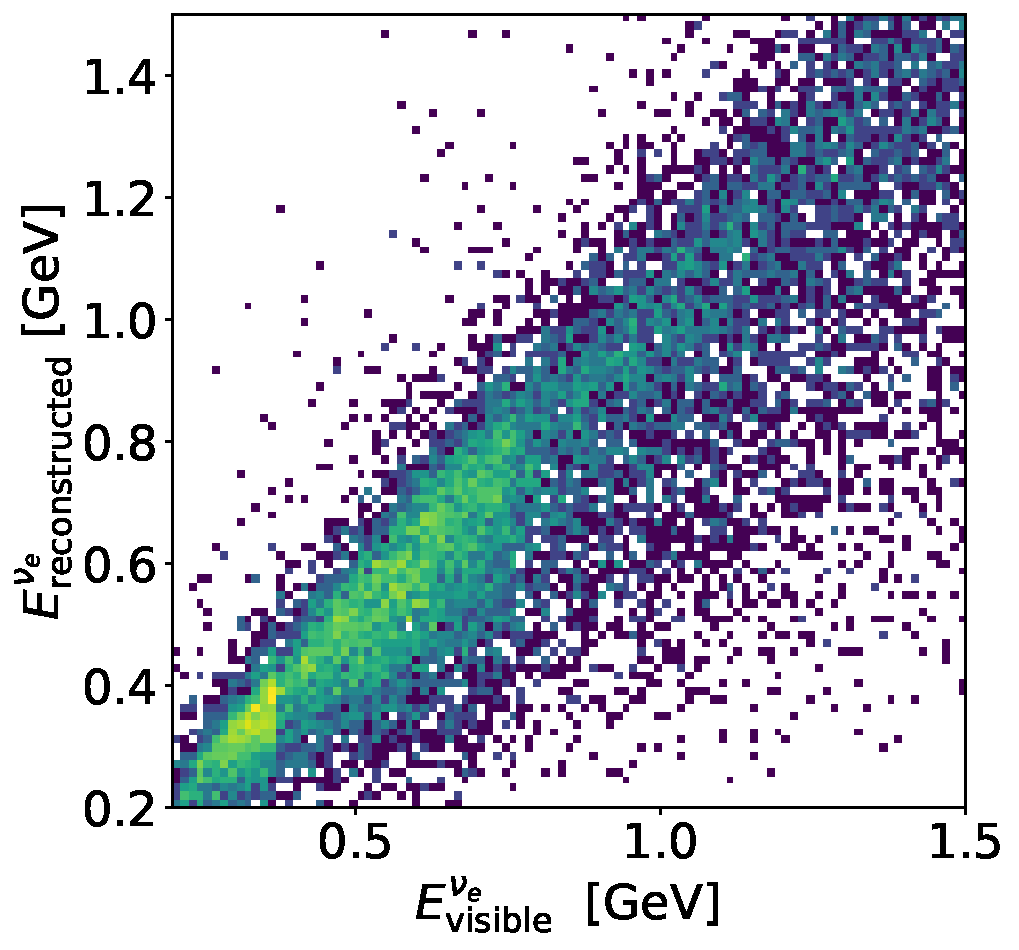
\includegraphics[width=1.00\textwidth]{ereco/nue_visible_eres2D.pdf}
    \caption{\label{fig:eres:nue:vstrue} }
    \end{subfigure}
\caption{\label{fig:eres:neutrino}Log-scale color-maps.}
\end{center}
\end{figure}
